\documentclass[10pt,oneside,a4paper]{article}
\usepackage[left=2cm,right=2cm,top=2cm,bottom=1cm,includeheadfoot]{geometry}
\usepackage{ngerman}
\usepackage[utf8]{inputenc}
% \usepackage{amsfonts,amssymb,amsmath,cancel,graphicx,textcomp}
\usepackage{amsfonts,amssymb,amsmath,graphicx,textcomp}
\usepackage{float}
\usepackage{color,xcolor}
\usepackage{url}
\usepackage{hyperref}
\usepackage{listings}
\usepackage{tikz}
\usepackage{fancyhdr}
\usetikzlibrary{arrows,shapes,snakes,automata,backgrounds,petri,positioning}

\hypersetup{
    colorlinks,
    citecolor=black,
    filecolor=black,
    linkcolor=black,
    urlcolor=black
}

\pagestyle{fancy}
\fancyhf{}
\fancyhead[L]{crash override : \\Steve Dierker, Semjon Kerner, Artur Jeske}
\fancyhead[C]{"Ubungsblatt 05}
\fancyhead[R]{Seite \thepage}
\renewcommand{\headrulewidth}{0.5pt}

% lstlisting mit Zeilennummerierung und grauen Kommentaren, Zeilenumbruch, etc. pp.
\lstset{
  numbers=left, numberstyle=\tiny, numbersep=5pt,
  tabsize=2,
  breaklines=true, breakindent=0pt, postbreak=\mbox{$\rightarrow\ \ $},
  showstringspaces=false,
  extendedchars=false,
  basicstyle=\small\ttfamily,
  commentstyle=\color{black!40},
  stringstyle=\color{black!40!blue},
  keywordstyle=\color{black!40!green}
}

% Komma Abstände bei Tausendern/Dezimalzahlen ans dt. anpassen
\mathcode`,="013B
\setlength{\parindent}{0em}
\setlength{\parskip}{0.5em}

\begin{document}
  \section{Aufabe 1}
    \begin{center}
      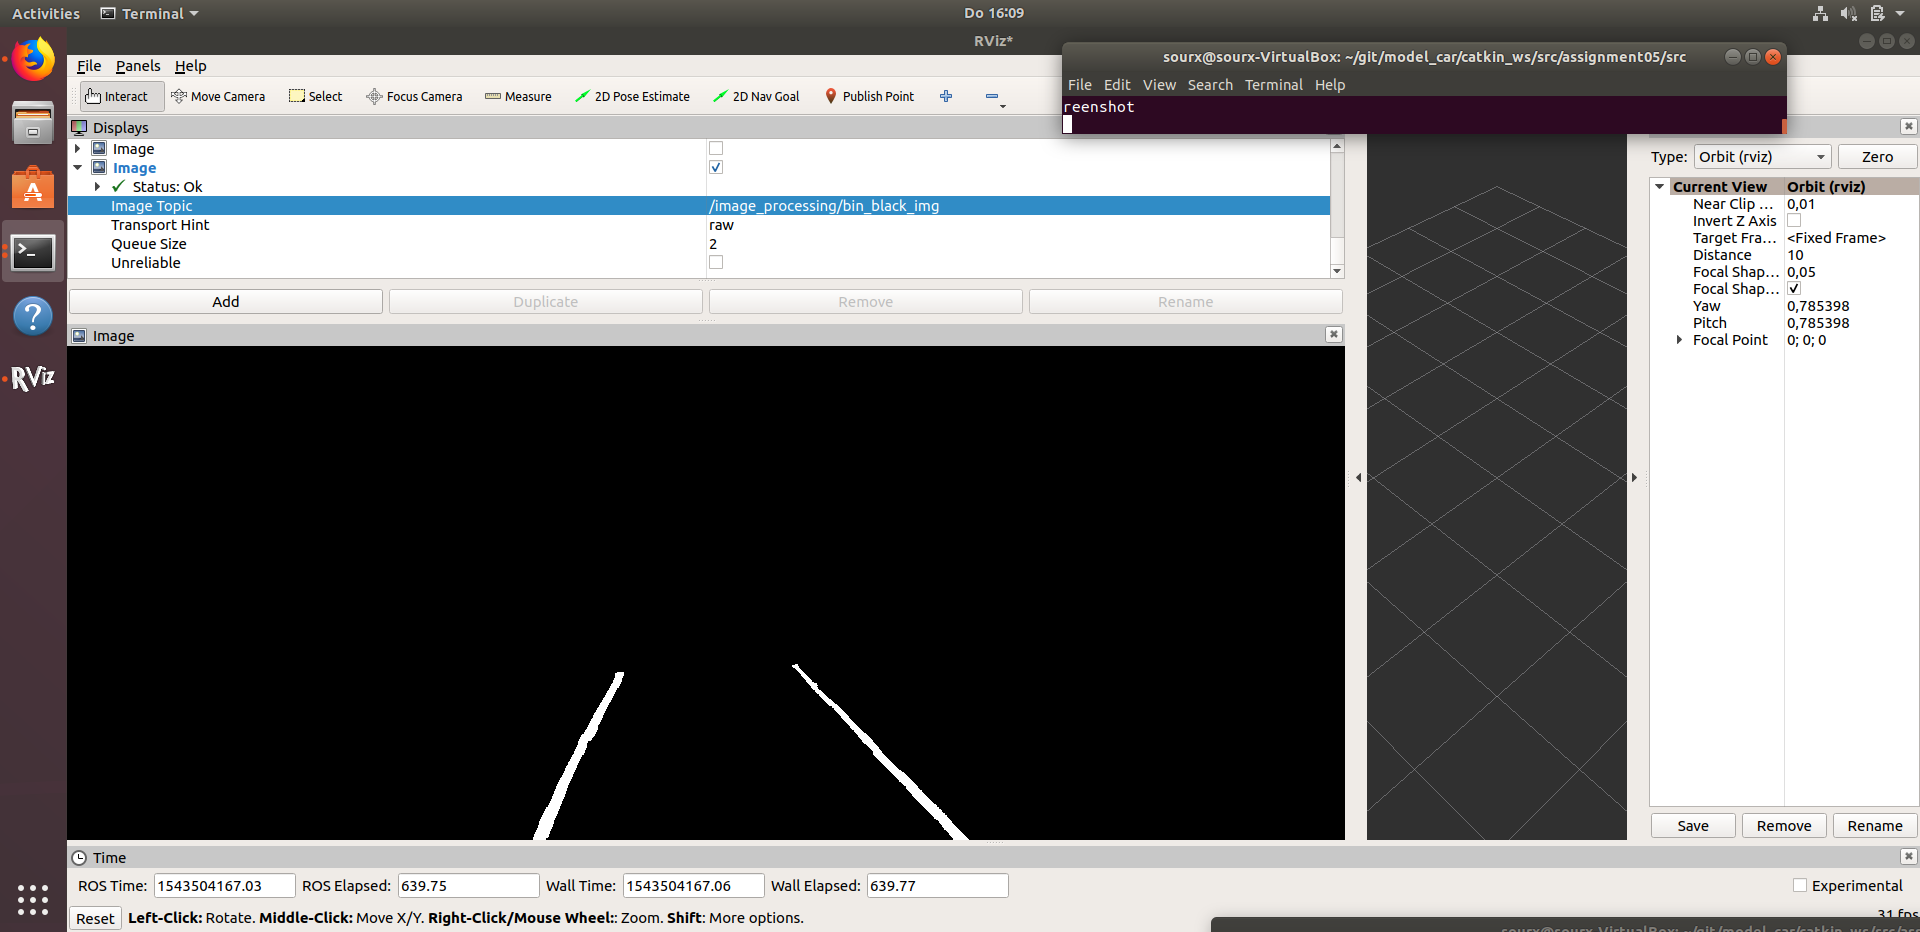
\includegraphics[scale=0.2]{pictures/assignment05_1.png}
    \end{center}
    See the code at the end.
  \section{Aufgabe 2}
    Sadly we had a lot of obstacles costing us hours of worktime, thus the code
    of the second Exercise is not debugged and may not work. It is very
    unfortunate that there is supposedly no tutor assigned on thursdays whom we
    could have asked for help and also the ros wiki was down from at least
    10:00 to 18:00 where we planned to have our main working time. Also the
    all the batteries were drained in the end and we could not test our programs
    on a running car, which of course may be prevented with proper rosbags in
    the future.\\

    \lstinputlisting[language=Python]{../catkin_ws/src/assignment5/src/lanesegment.py}
\end{document}
